% !TeX encoding = UTF-8
\section{Results}

% Description of input data
% Descriptive/explorative data analysis

On average a Mondrian paintings consist of 78.3\% colors (red, blue, yellow) and
21.7\% non-colors (black, white) ($\sigma = 17.2\%$), see Figure
\ref{fig:colors-noncolors}. The distribution of different colors appears to be
fairly uniformly distributed as you can see in Figure \ref{colors-rby}.

% Numbers close to Paretos Principle. But not quite: possibly 80% of the
% painting colors (Discussion)

\begin{figure}
  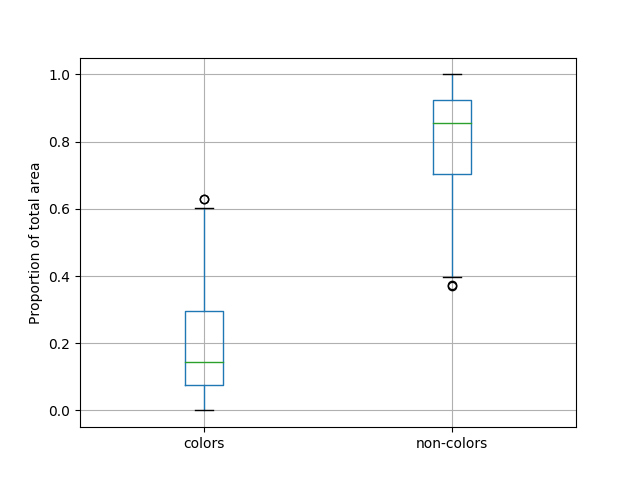
\includegraphics[width=\linewidth]{images/colors-non-colors.png}
  \caption{Percentage of color/non-color of the total area}
  \label{fig:colors-noncolors}
\end{figure}

\begin{figure}
  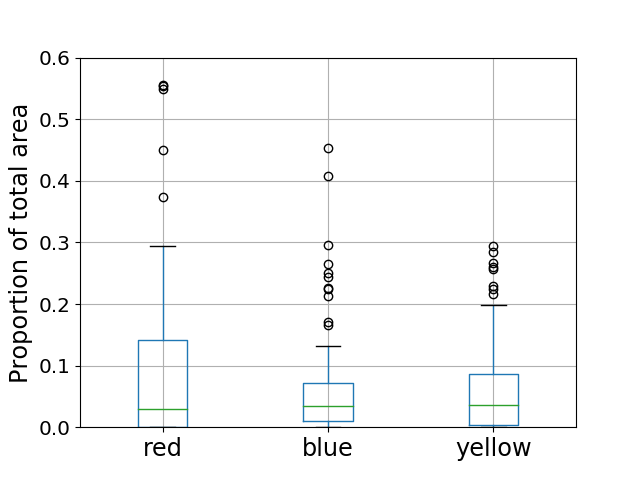
\includegraphics[width=\linewidth]{images/colors-rby.png}
  \caption{Percentage of red, blue and yellow of the total area}
  \label{fig:colors-rby}
\end{figure}

To see if different colors of rectangles have overall preferred positions in the
compositions, we assembled a dataset of all rectangles and their respective
positions, width and colors. We calculated the center of all of these rectangles
and plotted them by color. We also visualised the estimated probability density
function of the positions using Kernel density estimation. The first thing you
notice is that the color red appears to have a substantial bias to the top-left
corner. Similarly blue has a slighter bias to the bottom-right corner.

\begin{figure}
  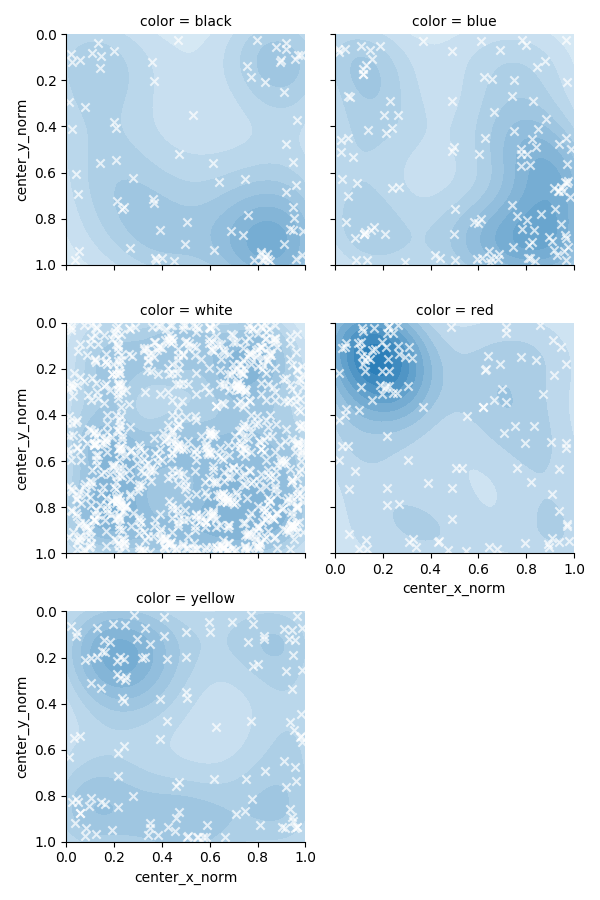
\includegraphics[width=\linewidth]{images/kernel-densities.png}
  \caption{Scatter plots and KDE for each color}
  \label{fig:kde}
\end{figure}

% Colors vs. non-colors (different colors)
% Ratios of rectangles
% Position of rectangle centers

% TODO: Number of rectangles over time?
% TODO: How many paintings use all colors? How many with only one?
